\section{Design}

%This is where the logical / abstract contribution of the project is presented.

%Notice that, when describing a software project, three dimensions need to be taken into account: structure, behaviour, and interaction.

%Always remember to report \textbf{why} a particular design has been chosen.
%Reporting wrong design choices which has been evalued during the design phase is welcome too.

In questa sezione esporremo il design del progetto, partendo dalle decisioni prese in ambito architetturale e proseguendo
col design di dettaglio.

\subsection{Structure}

Come menzionato nei precedenti capitoli, l'obiettivo del progetto è quello di fornire un meccanismo per realizzare sistemi multi-agente distribuiti in \textit{JaKTa}, ed
il gruppo ha deciso di conseguirlo fornendo un' estensione del framework il più minimale possibile.

Dal punto di vista architetturale, il progetto si colloca come modulo aggiuntivo del framework \textit{JaKTa}.

\begin{figure}[h]
    \centering
    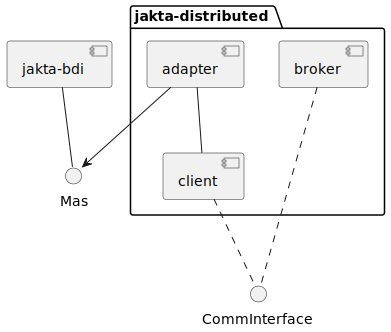
\includegraphics[width=0.8\textwidth]{figures/architecture.png}
    \caption{Architettura del progetto}
    \label{fig:architecture}
\end{figure}

\subsection{Design di dettaglio}

\subsubsection{Client}

L'applicativo del client è progettato per gestire la comunicazione attraverso WebSocket,
facendo uso del framework Ktor in Kotlin. Per affrontare la natura distribuita del progetto,
sono state definite entità chiave, tra cui \textit{Client}, \textit{WebSocketSession}, e i modelli di dati
\textit{SerializableSendMessage} e \textit{SerializableBroadcastMessage}. \\

L'interfaccia Client svolge il ruolo di punto principale di accesso, incapsulando le funzionalità fondamentali per la
comunicazione. La sua implementazione chiave è rappresentata dalla classe \textit{WebSocketsClient}.\\

La classe WebSocketsClient è una componente centrale per gestire le connessioni WebSocket.
È responsabile della creazione e gestione di sessioni WebSocket per la pubblicazione,
la sottoscrizione e la trasmissione di messaggi. Inoltre, tiene traccia delle connessioni attive, delle disconnessioni e dei messaggi in arrivo.\\

I modelli \textit{SerializableSendMessage} e \textit{SerializableBroadcastMessage} sono essenziali per rappresentare i messaggi scambiati tra il client e
il server. La loro struttura è progettata per garantire una corretta serializzazione e deserializzazione dei dati. \\

Vengono implementate tre funzionalità principali:
\begin{itemize}
    \item \texttt{publish}: si occcupa di inviare un messaggio ad un determinato 'topic' attraverso una connessione WebSocket;
    \item \texttt{broadcast}: simile alla funzione sopra citata ma è destinata ad unviare un messaggio a tutti i client connessi;
    \item \texttt{subscribe}: gestisce l'iscrizione del client ad un particolare 'topic' attraverso una connessione WebSocket.
\end{itemize}

Per quanto riguarda la gestione dei messaggi in arrivo, la funzione \texttt{subscribe}.
Questa funzione rimane in ascolto dei messaggi inviati al 'topic' specificato, deserializza i messaggi ricevuti e li memorizza per un successivo utilizzo.
Questo meccanismo è fondamentale per garantire una comunicazione bidirezionale efficace tra il client e il server.

%Which entities need to by modelled to solve the problem? 
%
(UML Class diagram)

%How should entities be modularised?
%
(UML Component / Package / Deployment Diagrams)

\subsection{Behaviour}

How should each entity behave?
%
(UML State diagram or Activity Diagram)

\subsection{Interaction}

How should entities interact with each other?
%
(UML Sequence Diagram)
